\section{Graphene on SGX}
\label{sec:eval:sgx}

%This section will shows the evaluation results of the \graphenesgx{} framework,
%in term of performance, security, and compatibility to Linux.

%\subsection{Performance Evaluation}
\label{sec:eval:perf}


%We evaluate the performance overheads on running unmodified Linux applications
%on SGX.
%Unlike the existing \sgx{} shielding systems which focuses on cloud-based systems or microservices,
\graphenesgx{} is designed to be general-purpose, supporting a broad range of
server and command-line applications. 
%, including both server and desktop workloads.
%\fixmedp{I wouldn't really call gcc or R ``desktop''}
\fixme{get rid of the part that we need to compile source code}
We thus evaluate performance overheads of unmodified Linux applications, using binaries 
from an Ubuntu installation.
%, or,
%in the case of Apache, Lighttpd, and NGINX,
%compiled from original source code using the default configurations.}
%(Apache, Lighttpd, and NGINX are compiled from source).} %\fixmedp{which apps are compiled?}
Depending on the workload, we measure application throughput or latency.
%According to the types of workloads, we design experiments to evaluate whether \graphenesgx{} can support applications with acceptable throughput or latency.

%All applications in our experiments are real, unmodified Linux applications,
%either directly taken from a disk with Ubuntu installation,
%or compiled using the default configuration given by the developers.
%No source code modification or change of compilation environment is required in the experiments.
%In our experiments, we either test on application binaries taken off-the-shelf from the Ubuntu {\tt APT} repositories,
%or applications that are built from the default configurations
%provided by the developers.
%Either source code modification or adjustment of the compilation environment is avoided in the setup of experiments.
%Our evaluation simulates the realistic results of running unmodified Linux applications in \graphenesgx{}.
%running Linux COTS applications on commodity hardware.

In order to differentiate SGX-specific overheads 
from Graphene overheads,
%, which also
%runs on a Linux host without SGX, 
we use both
Linux processes and \graphene{} on a Linux host without SGX as baselines
for comparison.
%Since a large portion of the \libos{} design is inherited from the \graphene{} \libos{},
%the performance impact of adopting \graphenesgx{} is largely affected by the design choices made in \graphene{}.
%In order to show the performance impact of \graphenesgx{} over \graphene{}, we use both native Linux and \graphene{} on a Linux host as the baselines for comparison.
Note that \graphene{} includes two optional kernel extensions:
one that creates a reference monitor to protect the host kernel from 
the library OS, and one that optimizes fork by 
with copy-on-write for large (page-sized) RPC messages.
%implementing a multi-page RPC
%abstraction.
Neither of these extensions are currently supported in \graphenesgx{}.
%so we measure baseline Graphene with these disabled.
% can be optionally run with a reference monitor for security isolation, and a bulk IPC abstraction for fork optimization.
%Since neither of the features is ported in \graphenesgx{},
%we mostly compare \graphenesgx{} to \graphene{} with these two features disabled,
%to show a more meaningful comparison.

% Put figures at the front
\begin{figure*}[t!]
\centering

\begin{minipage}{.3\textwidth}
\centering
\footnotesize
\includegraphics[width=\linewidth]{sgx/lighttpd-throughput-latency}\\
{\bf (a) Lighttpd (25 threads)}
\end{minipage}
\begin{minipage}{.3\textwidth}
\centering
\footnotesize
\includegraphics[width=\linewidth]{sgx/apache-throughput-latency}\\
{\bf (b) Apache (5 processes)}
\end{minipage}
\begin{minipage}{.3\textwidth}
\centering
\footnotesize
\includegraphics[width=\linewidth]{sgx/nginx-throughput-latency}\\
{\bf (c) NGINX (event-driven)}
\end{minipage}

\caption{Throughput versus latency of web server workloads, including Lighttpd, Apache, and NGINX, on native Linux, \graphene{}, and \graphenesgx{}.
We use an ApacheBench client to gradually increase load, and plot
throughput versus latency at each point.  Lower and further right
is better.
%\fixmedp{RB: Add another sentence or two to explain what the experiment is and how to interpret} }
}
\label{fig:server-throughput-latency}
\end{figure*}


\fixmedp{RA asks for a limitations section; I don't think we should do this, but the expensive stuff (events, fork, open) we should add as much as we can about what, if anything,  can be done about it, and what can't without more hardware}

\paragraph{Experimental setup.}

We use a Dell Optiplex 790 Small-Form Desktop,
with a 4-core 3.20 GHz Intel Core i5-6500 CPU (no hyper-threading, with 6MB cache),
8 GB RAM, and a 512GB, 7200 RPM SATA disk.
%We disable SpeedStep and TurboBoost to prevent interference.
The host OS is Ubuntu 16.04.4 LTS, with Linux kernel 4.4.0-21.
Each machine uses a 1Gbps Ethernet card connected to a dedicated local network.
We use version 1.8 of 
the Intel \sgx{} Linux SDK~\cite{intel-sgx-linux-sdk} and driver~\cite{intel-sgx-linux-driver}.
%We measure version 0.4beta of \graphene{}.

%Adding more detail of KVM environment
%Unless otherwise noted, \graphenesgx{} measurements include the Phosphor instrumentation.

\subsection{Server applications}

One deployment model for SGX is to host network services
on an untrusted cloud provider's hardware.
%To measure this case, 
We measure three widely-used Linux web servers, including {\bf Lighttpd}~\cite{lighttpd} (v1.4.35), {\bf Apache}~\cite{apache} (v2.4.18), and {\bf NGINX}~\cite{nginx} (v1.10).
%, to evaluate the performance of server-type workloads in \graphenesgx{}.
%These applications are all sophisticated, non-trivial workloads, and are constantly being used for commercial purposes.
%We test these applications to evaluating significantly different execution patterns, to benchmark the performance of \graphenesgx{} under each circumstances.
%Also, we do not explicitly configure these servers to secure their payloads using the HTTPS protocol.\fixme{if have time, maybe try again with HTTPS}
For each workload, we use ApacheBench~\cite{apachebench} to download the web pages on a separate machine.
%\edit{over Gigabit LAN}. %\fixmedp{more specific?}
%across a high-speed \fixmedp{Can you say
%more specifically the specs, like 10 GBps or whatever; also, if this is the same vlan, I might just describe this as being on a LAN, minimizing interference} University network.
The concurrency of ApacheBench is gradually increased during the experiment, to test the both the per-request latency and the overall throughput of the server.
Figure~\ref{fig:server-throughput-latency} shows the throughput versus latency of these server applications
in \graphenesgx{}, \graphene{} and Linux. 
Each workload is discussed below.

{\bf Lighttpd}~\cite{lighttpd} is a web server designed to be light-weight, yet robust enough for commercial uses. 
Lighttpd is multi-threaded; we test with 25 threads to process HTTP requests. 
By default, Lighttpd uses the \syscall{epoll\_wait} system call to poll listening sockets.
At peak throughput and load,  both \graphene{} and \graphenesgx{} have marginal overhead on either latency or throughput of the Lighttpd server.
The overheads of \graphene{} are more apparent when the system
is more lightly loaded, at 
%When Lighttpd is not overloaded, \graphenesgx{} causes 
15--35\% higher response time, or 13--26\% lower throughput. 
Without SGX, \graphene{} induces 
11--15\% higher latency or 13-17\% lower throughput over Linux;
the remaining overheads are attributable to SGX---either hardware or our OS shield.
%platform adaptation layer (PAL) code.

%\fixmedp{Some more detailed analysis would be nice.}
%Only part of this overhead is contributed by the library OS implementation, since using \graphene{} without \sgx{} causes only 

%\fixmedp{Why did you comment this out?  Let's discuss: Does it really make sense to have two points at the same  x-axis value?  Perhaps the axes should be inverted?  I'm not really sure about the methodology, but something about the line doubling back on itself seems wrong.  Maybe you want to separate these and show throughput vs. load, and a CDF of latencies?}


{\bf Apache}~\cite{apache} is one of the most popular production web servers. We test Apache using 5 preforked worker processes to service HTTP requests,
in order to 
to evaluate the efficiency of \graphenesgx{} across enclaves.
%n server, 
%In the experiment, the Apache server creates 5 preforked processes which coordinate on processing HTTP requests.
This application uses IPC extensively---the preforked processes of a server use a System V semaphore to synchronize on each connection.
%When receiving a connection, the preforked processes of Apache will coordinate among themselves using the system V IPC semaphores.
Regardless of the workload, the response time on \graphenesgx{} is 12--35\% higher than Linux, due to the overhead of coordination across enclaves over encrypted RPC streams.
The peak throughput achieved by Apache running in \graphenesgx{} is 26\% lower than running in Linux.
In this workload, most of the overheads are SGX-specific, such as exiting enclaves when accessing the RPC, as non-SGX Graphene
has only 2--8\% overhead compared to Linux.

%The enclave restriction \fixmedp{Huh?} is the main contributor to this overhead, as \graphene{} generally only causes 2--8\% overhead.

%\fixmedp{Check the lightttp graph; the lines are right on top of each other, and dont' look 22\% apart to me.  Some of this may be the scale of the y axis}

{\bf NGINX}~\cite{nginx} is a relatively new web server designed for high programmability, for as a building block to implement different services.
Unlike the other two web servers, NGINX is event-driven and mostly configured as single-threaded.
%When running as a simple HTTP server, NGINX uses an event-driven model instead of multi-threading/multi-processing to handle incoming requests.
\graphenesgx{} currently only supports synchronous I/O at the enclave boundary,
and so, under load, it cannot as effectively overlap I/O and computation
as other systems that have batched and asynchronous system calls.
%Asynchronous system calls and events in general are less mature features of
%\graphenesgx{}, and, 
Once sufficiently loaded, NGINX on both \graphene{} and \graphenesgx{} 
performs worse than in a  Linux process. % once sufficiently loaded.
%We observe that both \graphene{} and \graphenesgx{} tend to perform poorly in an event-driven server.
The peak throughput of \graphenesgx{} is 1.5$\times$ lower than Linux;
without SGX, Graphene only reaches 79\% of Linux's peak throughput.
%\fixmedp{Maybe shout out to eleos, or cite other work}
We expect that using tools like Eleos~\cite{orenbach17eleos} to reduce exits
would help this workload; in future work, we will improve
asynchronous I/O in \graphenesgx{}.

%\graphenesgx{} causes 17--90\% more response time when the server is not overloaded,
%but up to 1.5$\times$ at the peak throughput.
%If we compare the peak throughput with native Linux, \graphenesgx{} is 70\% less.
%\graphene{} also suffers the same performance pattern, as the throughput drops dramatically after reaching 79\% of the peak throughput of NGINX in Linux.
%The reason of the slowdown is that the host interface of \graphene{} and \graphenesgx{} only supports synchronous IO, so implementing asynchronous IO will be less efficient. This limitation is a trade-off to the portability of \graphene{}.
%\fixmedp{Didn't get the portability point; please spell out what you meant, if important}

\begin{figure*}[t!]
\centering

\begin{minipage}{.4\textwidth}
\centering
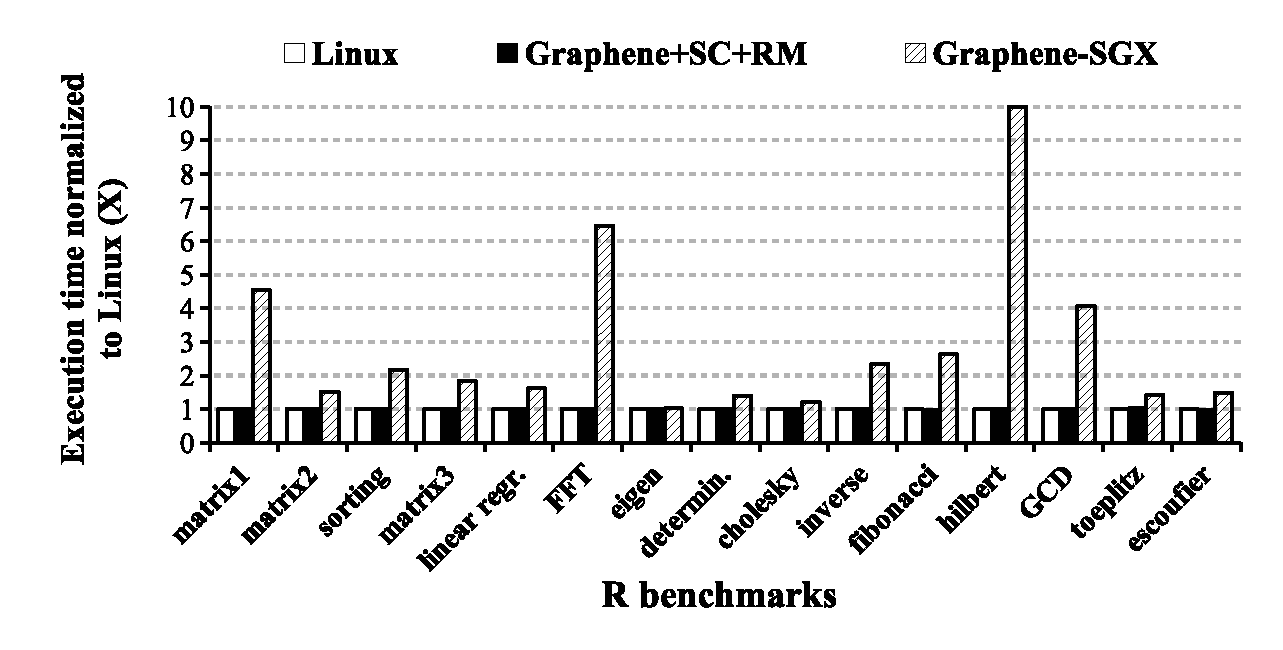
\includegraphics[width=\linewidth]{sgx/r-overhead}\\
{\bf (a) R}
\end{minipage}
\begin{minipage}{.275\textwidth}
\centering
\includegraphics[width=\linewidth]{sgx/gcc-overhead}\\
{\bf (b) GCC}
\end{minipage}
\begin{minipage}{.25\textwidth}
\centering
\includegraphics[width=\linewidth]{sgx/curl-overhead}\\
{\bf (c) CURL}
\end{minipage}

\caption{Performance overhead on desktop applications, including latency of R, execution time of GCC compilation, download time with CURL. The evaluation compares native Linux, \graphene{}, and \graphenesgx{}.} %{\bf Enclave creation time is deducted from the GCC execution time.}}
\label{fig:desktop-overhead}
\end{figure*}



\subsection{Command-Line applications}


We also evaluate the performance of a few commonly-used command-line applications.
%, to evaluate the performance of \graphenesgx{} on PCs instead of servers and clouds.
Three off-the-shelf applications are tested in our experiments:
{\bf R} (v3.2.3) for statistical computing~\cite{r-project}; {\bf GCC} (v5.4), the general GNU C compiler~\cite{gcc}; {\bf CURL} (v7.74), the default command-line web client on UNIX~\cite{curl}.
These applications are chosen because they are frequently used by Linux users,
and each of them potentially  be used 
in an enclave to handle sensitive data---either on a server or a client
machine.
% can realize profitable scenarios of using enclaves on desktop machines.



We evaluate the latency or execution time of these applications. 
%, because desktop users tend to care more about responsiveness than throughput.
In our experiments, both R and CURL have internal timing features to measure the wall time
of individual operations or executions.
%However, for other applications like GCC which does not include internal timing, evaluating the execution time can be influenced by many factors.
On a Linux host, the time to start a library OS is higher than a simple 
process, but significantly lower than booting a guest OS in a VM or
starting a container. 
Prior work measured Graphene (non-SGX) start time at 641 $\mu$s~\cite{tsai14graphene}, whereas starting an empty Linux VM takes 10.3s and starting a Linux (LXC) container takes 200 ms~\cite{agarwal15container}. 
%% dp; Note that this is MILLI seconds, not micro seconds.
%average memory footprint of an empty Linux VM, with memory deduplication, is about 96MB, . 


On SGX, the enclave creation time is relatively higher, \fixme{added more detailed number} ranging from 0.5s (a 256MB enclave) to 5s (a 2G enclave), which is a fixed cost that any application framework
will have to pay to run on SGX.
%For library OSes, the time for creating and initializing an enclave is not trivial, because it is similar to booting an lightweight OS.
% a significant part of the start-up time
% of an application is more significant, because creating enclaves is expensive.
%We consider the enclave creation time as a fixed cost for any application running in \graphenesgx{},
%and acceptable to users as long as it is responsive.
Enclave creation time is determined by the latency of the hardware and the Intel kernel driver, and is primarily a function of the size of 
the enclave, which is specified at creation time because it affects the enclave signature. %\fixmedp{although can't it grow with eadd?}.  
For non-server workloads that create multiple processes during execution,
such as GCC in Figure~\ref{fig:desktop-overhead},
the enclave creation contributes a significant portion to the execution time overheads, illustrated as a stacked bar.
%Since the enclave creation time is related to the enclave size, and unrelated to the workload,
%we deduct the enclave creation time from the execution time of GCC in Figure~\ref{fig:desktop-overhead}. \fixmedp{I think it might be better to show this as a stacked bar instead of just removing it.  Opaquely subtracting this cost doesn't seem right.  Let's discuss dp: I thought we agreed to change this...}

{\bf R}~\cite{r-project} is a scripting language often used for
data processing and statistical computation.
With enclaves, users can process sensitive data on an
OS they don't trust.
We use an R benchmark suite developed by Urbanek et al.~\cite{r-benchmark-25}, which includes 15 CPU-bound workloads such as matrix computation and number processing.
\graphenesgx{} slows down by less than 100\% on the majority of the workloads, excepts the ones which involve allocation and garbage collection: ({\tt matrix1} creates and destroys matrices, and both {\tt FFT} and {\tt hilbert} involve heavy garbage collection.)
Aside from garbage collection, these R benchmarks do not frequently interact with the host.
We further note that non-SGX \graphene{} is as efficient as Linux on all workloads, 
and these overheads appear to be SGX-specific.
%\fixmedp{Check this pontification}
In our experience, garbage collection and memory management code in managed language runtime
systems tends to be written with assumptions that do not match enclaves,
such as a large, sparse address space or that memory can be demand paged 
nearly for free (SGX version 1 requires all memory to be mapped
at creation); a useful area for future work would be to design
garbage collection strategies that are optimized for enclaves.
%we believe the overheads on \graphenesgx{} are contributed by enclaves.
 
{\bf GCC}~\cite{gcc} is a widely-used C compiler.
By supporting GCC in enclaves, developers can compile closed-source applications on customers' machines,
without leaking the source code.
GCC composes of multiple binaries, including {\tt cc1} (compiler), {\tt as} (assembler), and {\tt ld} (linker).
Therefore, GCC is a multi-process program using \syscall{execve}.
We test the compilation of thee source files with varied sizes,
using single C source files collected by MIT~\cite{gcc-benchmark}.
Each GCC execution typically \fixme{it's five, not four} creates five processes, and we run each process in a 256MB enclave by default.
%and has a fixed cost on enclave creation, which is unrelated to workload and depends on the enclave size.
%\fixme{check this}
\fixme{clarified this part, to prevent confusion between latency and overhead. also, GCC numbers got better.}
For a small workload like compiling {\tt gzip.c} (5 kLoC), running in \graphenesgx{} (4.1s) is 18.7$\times$ slower than Linux (0.2s).
The bulk of this time is spent in enclave creation, taking 3.0s in total, while the whole execution inside the enclaves, including initialization of the library OS and OS shield, takes only 1.1s, or 4.2$\times$ overhead.
For larger workloads like {\tt oggenc.c} (50 kLoC) and {\tt gcc.c} (500 kLoC), 
the overhead of \graphenesgx{} is less significant. % (3.6$\times$ and 2.1$\times$ overhead, respectively).
For {\tt gcc.c} (500 kLoC), we have to enlarge one of the enclaves ({\tt cc1}) to 2GB,
but running on \graphenesgx{} (53.1s) is only 2.1$\times$ slower than Linux (17.2s),
and 7.1s is spent on enclave creation.
%and the creation of four enclaves takes 8s.
%Each compilation has a fixed enclave creation time in \graphenesgx{}, which is about 1--2 seconds per enclave. We deduct the creation time of all enclaves  to gain more meaningful results, but do not hide rest of the overhead on fork.
%\fixmedp{Also not comfortable with this; add a bar?}
%In general, GCC in \graphenesgx{} is 1--5$\times$ slower than GCC on native Linux. 
%\fixmedp{This really needs some profiling if possible}
The overhead of non-SGX \graphene{} on GCC is marginal.
 



{\bf CURL}~\cite{curl} is a command-line  web downloader.
\graphenesgx{} can make CURL into a secure downloader that attests both server and client ends.
We evaluate the total time to download a large file, ranging from 1MB to 1GB, from another machine running Apache. % over Gigabit LAN.
%across high-speed university network\fixmedp{more specific, as above}.
\graphene{} has marginal overhead on CURL, and
\graphenesgx{} adds 7--61\% overhead to the downloading time of CURL, due to the latency of I/O.


\begin{figure*}[t!]
\centering

\begin{minipage}{.3\textwidth}
\centering
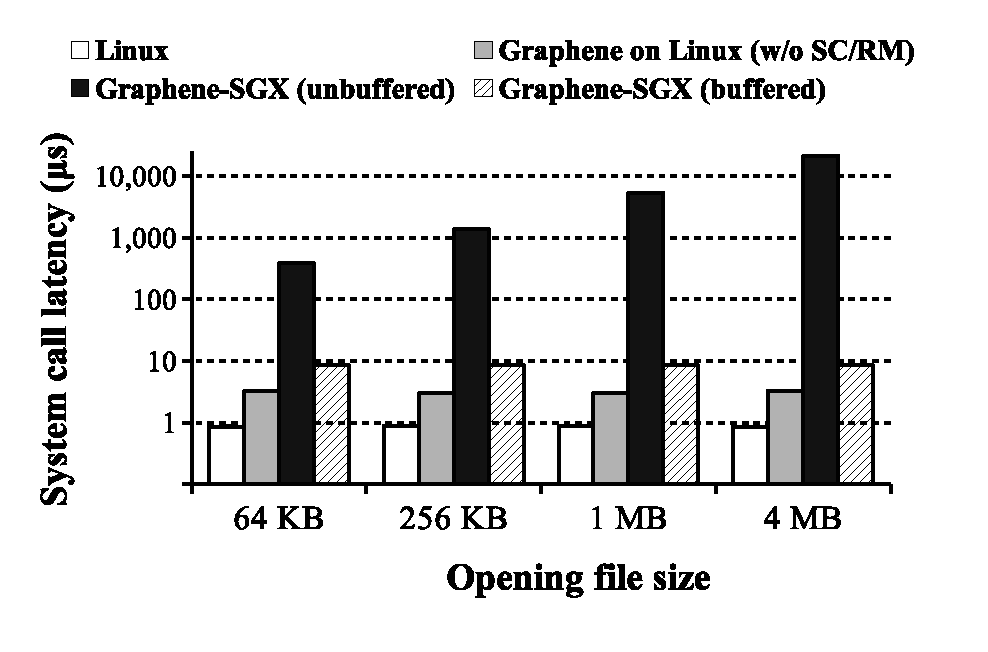
\includegraphics[width=\linewidth]{sgx/open-latency}\\
{\bf (a) Open a file}
\end{minipage}
\begin{minipage}{.3\textwidth}
\centering
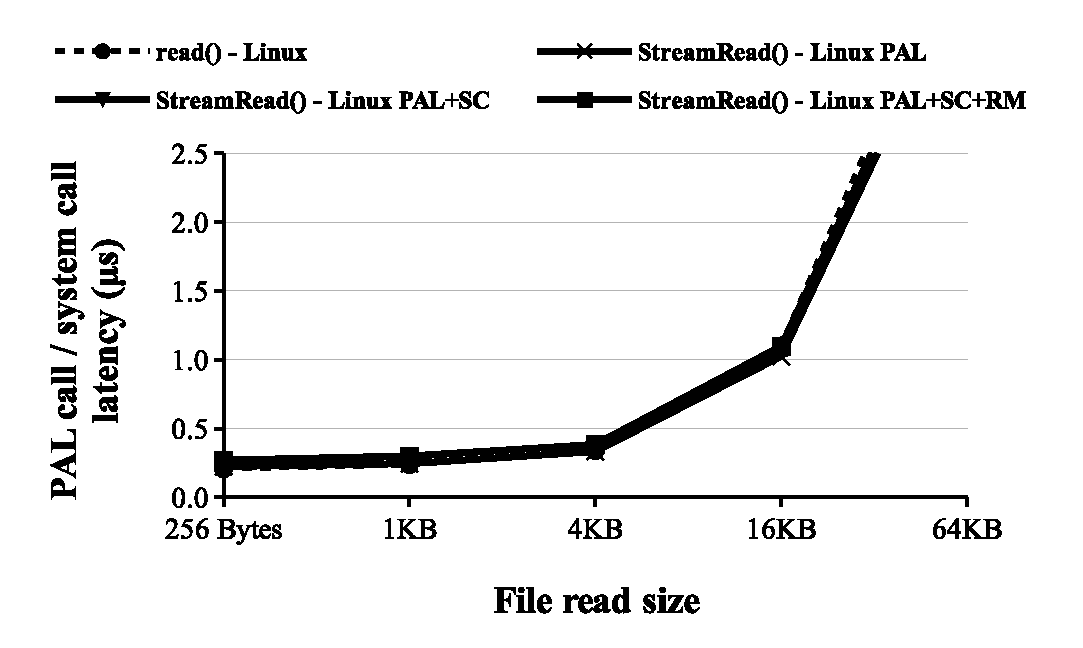
\includegraphics[width=\linewidth]{sgx/read-latency}\\
{\bf (b) Read a file}
\end{minipage}
\begin{minipage}{.3\textwidth}
\centering
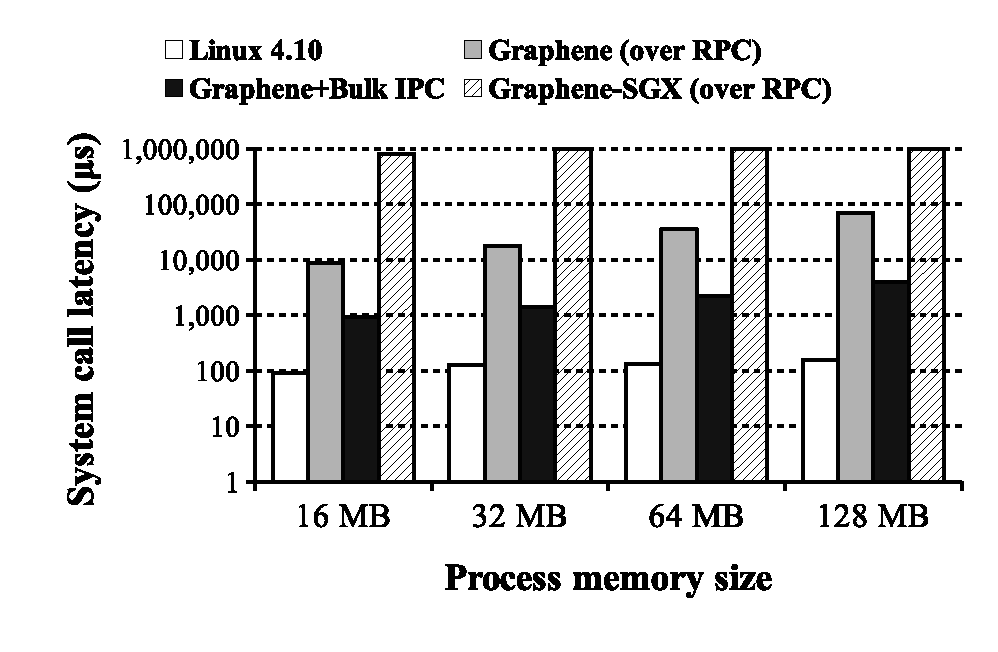
\includegraphics[width=\linewidth]{sgx/fork-latency}\\
{\bf (c) Fork a process}
\end{minipage}

\caption{Latency of some expensive system calls in \graphenesgx{}, including opening and reading a secured (authenticated) file, and forking a new process. The results are compared with native Linux and \graphene{}.}
\label{fig:syscall}
\end{figure*}


\subsection{Performance Overhead Analysis}


In this section we evaluate a few system operations that are heavily impacted by the \graphenesgx{} design.
%To shield dynamic loading and process creation,
%\graphenesgx{} uses computationally-expensive cryptographic techniques \fixmedp{more specific?} to verify enclave inputs.
% under the circumstance that the host OS cannot be trusted.
%As a trade-off to the security, the performance will be affected
%by additional cryptographic computation.
We measure the \syscall{open}, \syscall{read}, and \syscall{fork} system calls
using LMbench 2.5~\cite{McVoy:lmbench}.
A primary source of the overheads on these system calls is the cost of shielding applications, with run-time checks on the inputs.
Cryptographic techniques are used to: (1) validate the file against the secure hash, at \syscall{open}, (2) check the file chunks against the Merkle tree, at \syscall{read}, and (3) establish a TLS connection over inter-enclave RPC, at \syscall{fork}.
%opening a integrity-sensitive file for the first time, 
% or using cryptographic techniques, such as secure hashing, to verify the inputs.
% microbenchmarking specific system calls: 
% system calls,
%with different application settings.
%The microbenchmark is part of the LMBench 2.5 test suite
%\fixmedp{maybe merge this in the above paragraph, which feels a little coy}
%For instance, in order to shield dynamic loading, \graphenesgx{} checks each binary file against the secure hashes in the manifest,
%when the file is opened for the first time---after the whole file is copied into the enclave.
%\fixmedp{This happens after they are copied into enclave, memory right?}
%The verification happens when opening the file for the first time (often by the 
%After \graphenesgx{} validates the file, we generate a series of hashes of the file in chunks, as a merkle tree.
%to prevent verifying the whole file again when later randomly reading a part of the file.
%\fixmedp{So is this for the case when a file is swapped out?  I'm confused here - some details are missing}
%The latency of opening and reading an authenticated file in \graphenesgx{} is dominated by SHA256 and SHA512 calculation.
The remaining overheads contribute to exiting the enclave for host system calls, and bringing memory into the EPC (enclave page cache) or decrypting 
memory on a last-level cache miss. %and later the cache where the memory is decrypted by the CPU.


Figure~\ref{fig:syscall}(a)
shows the overhead for authenticating files in \syscall{open}.
\fixme{change overhead to latency}
Depending on the file size, the latency of \syscall{open} on \graphenesgx{} is 383$\mu$s (64KB file) to 21ms (4MB file), whereas on Linux, the latency is constant at 0.85$\mu$s.
We note that this is where enclaves are at a disadvantage, as \syscall{open} 
normally does not need to read file content; whereas here \graphenesgx{} uses \syscall{open}
as a point at which to validate file content.
For a subsequent \syscall{open}, when the Merkle tree is already generated, the overhead of simply exiting enclave for \syscall{open}, and searching the file list in the manifest, is about 9$\times$.
%\fixmedp{why?}


One might be able to optimize further for cases where only part of a file is accessed
with incremental hashing.  However, in the common case where nearly all of the file is accessed,
these costs are difficult to avoid when host file system is untrusted.
Another opportunity 
is to create the Merkle tree offline, when the manifest is created.
%\fixmedp{I think the second idea has legs...}


%This is an inevitable cost, because normal \funcname{open} on trusted OSes
%need not to access file content.
%After verifying the file, \graphenesgx{} buffers the chunk hash values, to skip whole-file verification when the file is reopened.

Figure~\ref{fig:syscall}(b)
shows the overhead for authenticating files in \syscall{read}, which 
is lower than \syscall{open}.
Since the whole file has been verified at \syscall{open}, the sequential \syscall{read} only verifies the chunks of files it is reading from untrusted memory.
%Reads from data cached in enclave memory are cheaper.  %\fixmedp{right? can we say how much cheaper?  Maybe add separate bars for both cases?}
% Therefore, \syscall{read} is actually much cheaper than \syscall{open}.
Depending on the size of blocks being read, the latency on \graphenesgx{} is 0.5$\mu$s (64-byte \syscall{read}) to 16.9$\mu$s (4KB \syscall{read}). The latency of \syscall{read} on Linux is \roughly{}0.1$\mu$s for any block size below 4KB.
If the file is not authenticated,
\graphenesgx{} only copies the file contents into the buffer, and the overhead reduces to 48\% (64-byte \syscall{read}) to 83\% (4KB \syscall{read}).
\fixmedp{Consider doing larger buffers, say up to 64k or even 4 MB}

%\fixmedp{In the legend for 7b, unsecure should be insecure}


Figure~\ref{fig:syscall}(c) shows the overhead of forking a process.
As described in \ref{sec:multiproc}, the latency of \syscall{fork} in \graphenesgx{} is affected by three factors:
creation of a new enclave, local attestation of the integrity, and duplicating the process state over an encrypted RPC stream.
Combining these factors, \syscall{fork} is one of the most expensive calls in \graphenesgx{}.
%, but at least it is supported natively on the current hardware.
The default enclave size is 256MB.
%which takes \roughly{}0.5s to create. 
Our evaluation shows that the latency of forking a process is around 0.8s (16MB process) to 2.7s (128MB process), but can be more expensive if the parent process uses more memory.
The trend matches the performance of \graphene{} without the bulk IPC optimization.
\fixmedp{If you want, some thoughts on how this might be improved in the future would be nice...  One good suggestion is recycling enclaves, or pre-forking so measurements can be done in parallel}
%Due to the overhead on \funcname{fork}, \graphenesgx{} is not suitable for fork-intensive workloads like Bash scripts
%if performance is critical.

\fixme{talk about a limitation of improving fork. check this.}
One way to further optimize \syscall{fork} is to reduce or avoid enclave creation time; one can potentially pre-launch a child enclave, and then migrate the process contents later when \syscall{fork} is called.
There might be another opportunity to improve the latency of process migration,
if copy-on-write sharing of enclave pages can be supported in future generations of SGX.
%Unfortunately, sending the process contents is difficult to avoid in \syscall{fork},
%as SGX disallows sharing enclave memory between multiple enclaves.

%\fixmedp{I assume 5.4 isn't done yet}



\subsection{TCB Size and Shielded Functionality}

In this section we measure the increase in TCB size of \graphenesgx{},
%in lines of code, 
as well as 
%compare the TCB size increased by \graphenesgx{} to an unmodified application, in lines of code, and 
the OS functionality shielded by the framework.
We compare to \scone{} and \panoply{}, using
%For SCONE and Panoply, we use 
numbers reported in their papers. 
%The conventional One generally assumes 
A smaller TCB is generally easier to review or possibly verify,
and is assumed to have fewer vulnerabilities.
%more implies lower burden for code review or formal verification, and less risk of writing exploitable code.
%For instance, Panoply argues that, because its use cases are typically smaller than 20kLoC, including both the application logic and Panoply itself, it is within the realm of future, automated verification~\cite{shinde17panoply}.

\fixmedp{Reviewer B asks for memory footprint, which isn't a bad idea}

\begin{table}
\footnotesize
\centering
\bgroup
\def\arraystretch{1.2}
\setlength{\tabcolsep}{0.5em}
\begin{tabular}{>{\raggedright\arraybackslash}p{9em}>{\raggedleft\arraybackslash\bf}p{7em}>{\raggedleft\arraybackslash}p{4.25em}>{\raggedleft\arraybackslash}p{4.25em}}
Components                    & \graphenesgx{}  & \scone{}     & \panoply{}  \\
\hline
libc (ld, libm, pthread)      &  1,292 &   88 & --      \\
                              & (glibc-2.19) & (musl)   &          \\
Library OS                    &     34 &  --      & --     \\
PAL / OS Shield               &     22 &   99 & 10  \\
\hline
Total                         &  1,348 &  187 & 10  \\
\hline
\end{tabular}
\egroup
\caption{TCB size (in thousands of lines of code) of \graphenesgx{}, \scone{}, and \panoply{}.}
\label{tab:tcb-size}
\end{table}

Table~\ref{tab:tcb-size} lists the lines of code in each components within the TCB of \graphenesgx{}, \scone{}, and \panoply{}.
By comparing the total TCB size, \graphenesgx{} is 9$\times{}$ larger than \scone{}, and 134$\times{}$ larger than \panoply{}.
However, the primary difference is the selection of libc: 
for maximum compatibility, \graphene{} uses glibc.
\scone{} uses the smaller musl libc, which lacks some features of glibc.
%it would be easy to use the smaller, and incomplete, musl libc.
%SCONE uses 
% Linux applications, \graphenesgx{} chooses to use a minimally-modified glibc, whereas SCONE uses the much more lightweight musl and 
\panoply{} excludes libc from its TCB,
% \fixmedp{what is their rationale, again? Check this}
to fit into the range of automated formal verification,
as they shield at the libc interface.
In principle, \graphene{} could easily support musl as well as glibc for applications
that do not need the additional features of glibc.
We also see the benefit of removing unused code from 
libraries, especially in an unsafe language,
similar to the approach taken in unikernels~\cite{unikernels}.
On balance, 
this choice of libc implementation is largely orthogonal to the issue
of how general-purpose the shields are.

%We argue that the choice of libc is orthogonal to the design of \graphenesgx{}; one can statically compile the applications against musl or glibc if TCB size is a concern, or given plenty of time, trim the libc functionality to bare minimum. 

If we focus on the TCB size of the library OS and the shields, 
\graphenesgx{} is 
%library OS and PAL in \graphenesgx{}, with the shielding layer of SCONE, we are 
44\% smaller than \scone{}. 
We cannot analyze the size of \scone{} because it is closed source.
%, although
%we suspect
%Although it is unclear what is in the implementation of SCONE, because it is not yet open-sourced, we believe the largest portion of their TCB contributes to the cryptography library.
\panoply{} has a smaller TCB in its shield, but within the same order of magnitude.
Panoply only shields 91 out of 256 supported POSIX functions; for context, POSIX 1003.1 defines 1,191 APIs~\cite{POSIX1003-1-2008}.
%out of 256 currently supported by \panoply{} \fixmedp{The better number is how many total functions in POSIX}.

All three of these compatibility layers or shields are within the same
order of magnitude in code size, and the differences are likely 
correlated with different ranges of supported functionality.
A recent study indicates that only order-of-magnitude differences in code
size correlate with reported CVE vulnerabilities; within the same order-of-magnitude,
the data is inconclusive that there is a meaningful difference in risk~\cite{security-metric}.
Thus, increased generality does not necessarily come with 
increased risk. % is not a clear relationship between risk 

% data only correlates
%with differences in code size when 

%Besides the choice of libc, we argue that the TCB size of a library OS or a shim shielding layer is actually correlated with the functionality that it supports or shields. Because none of the three frameworks have completely shielded the whole Linux system call table or POSIX, it is unclear how much code has to be added in the future. \graphenesgx{} also shows that one can always engineer a library OS with a small TCB, if most code is not reused from a monolithic OS kernel like Windows or Linux.
%A recent study of the CVE database also points out that having a larger TCB does not necessarily indicate more vulnerabilities, even when the difference is more than two order-of-magnitude. 


